\documentclass[../../main.tex]{subfiles}
\begin{document}

{\bf [解]}
円の半径を $1$ として考えて良い．この円に内接する正 $k$ 角形の面積 $S_k$ は,
図のように高さ$\cos \dfrac{\pi}{k}$，底辺$2\sin \frac{\pi}{k}$の三角形が$k$個あるとして計算できるから
\begin{align}
S_k 
 & = k \cdot \frac{2\sin \frac{\pi}{k} \cos \frac{\pi}{k}}{2} \\
 & = \frac{k}{2} \sin \frac{2\pi}{k} \label{eq:1}
\end{align}
とかける．

\begin{figure}[htb]
\begin{center}
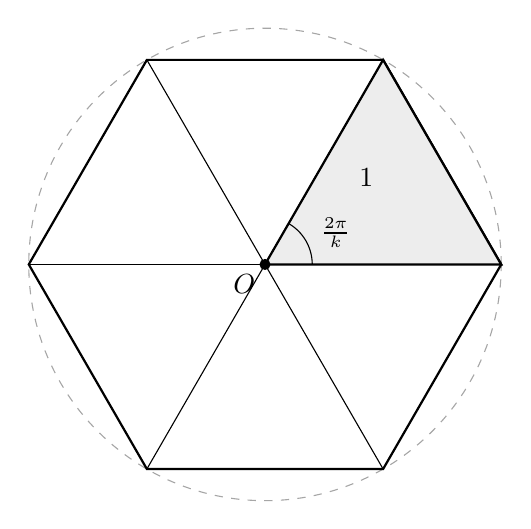
\begin{tikzpicture}[scale=2, >=stealth]
  % 外接円の描画（破線）
  \draw[dashed, gray!70] (0,0) circle (1.5cm);

  % 各頂点の定義 (半径1.5, 60度刻み)
  \foreach \i in {1,...,6} {
    \coordinate (P\i) at ({60*\i - 60}:1.5);
  }

  % 正六角形の描画
  \draw[thick] (P1) -- (P2) -- (P3) -- (P4) -- (P5) -- (P6) -- cycle;

  % 中心から各頂点への線分（6つの三角形をつくる）
  \foreach \i in {1,...,6} {
    \draw (0,0) -- (P\i);
  }

  % 1つの三角形（第1象限の三角形）を薄く塗りつぶして強調
  \fill[gray!20, opacity=0.7] (0,0) -- (P1) -- (P2) -- cycle;
  \draw[thick, fill opacity=1] (0,0) -- (P1) -- (P2) -- cycle;

  % 中心 O と半径 1 の表示
  \fill (0,0) circle (1pt) node[below left] {$O$};
  \node[above left] at (0.75, 0.43) {$1$};

  % 中心角 (2π/k = 2π/6 = π/3) の表示
  \draw (0.3,0) arc (0:60:0.3);
  \node at (0.45, 0.2) {\small $\frac{2\pi}{k}$};

\end{tikzpicture}
\end{center}
\caption{円に内接する正六角形とそれを構成する $k=6$ 個の三角形}
\end{figure}

\begin{figure}[htb]
\begin{center}
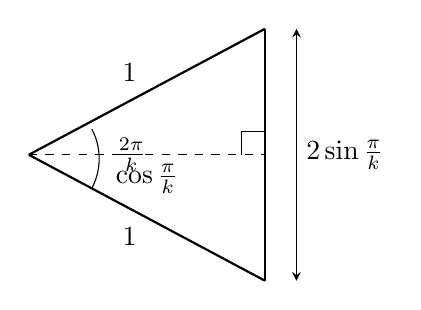
\begin{tikzpicture}[scale=2, >=stealth]
  % 頂点
  \coordinate (O) at (0,0);
  \coordinate (A) at (1.5, 0.8);
  \coordinate (B) at (1.5, -0.8);
  \coordinate (M) at (1.5, 0); % 底辺の中点

  % 三角形 OAB
  \draw[thick] (O) -- (A) node[midway, above left] {$1$};
  \draw[thick] (O) -- (B) node[midway, below left] {$1$};
  \draw[thick] (A) -- (B);

  % 垂直二等分線（高さ）
  \draw[dashed] (O) -- (M) node[midway, below] {$\cos \frac{\pi}{k}$};

  % 直角マーク
  \draw (1.35, 0) -- (1.35, 0.15) -- (1.5, 0.15);

  % 角の弧とラベル
  \draw (0.4, -0.213) arc (-28.07:28.07:0.4);
  \node at (0.65, 0) {$\frac{2\pi}{k}$};

  % 底辺の長さのラベル
  \draw[<->] (1.7, -0.8) -- (1.7, 0.8) node[midway, right] {$2\sin \frac{\pi}{k}$};
\end{tikzpicture}
\end{center}
\caption{正 $k$ 角形を構成する二等辺三角形}
\end{figure}


従って題意の不等式に\cref{eq:1}を代入すると
\begin{align}
    &\frac{2}{3} S_{3n} < S_n < \frac{\sqrt{3}}{2} S_{2n} \\
    \iff &\frac{2}{3} \cdot \frac{3n}{2} \sin \frac{2\pi}{3n} < \frac{n}{2} \sin \frac{2\pi}{n} < \frac{\sqrt{3}}{2} \cdot \frac{2n}{2} \sin \frac{2\pi}{2n} \\
    \iff &\sin \frac{2\pi}{3n} < \frac{1}{2} \sin \frac{2\pi}{n} < \frac{\sqrt{3}}{2} \sin \frac{2\pi}{2n} \qquad \dots \text{\textcircled{1}} \label{eq:2}
\end{align}
である．そこで以下\cref{eq:2}を満たす$n$を求める．

まずは\cref{eq:2}の左側の不等号から考える．
簡単のため $t = \sin \frac{2\pi}{3n}$ とおくと三倍角の公式から
\begin{align}
 \sin \frac{2\pi}{n} = 3t - 4t^3
\end{align}
だから\cref{eq:2}の左側は
\begin{align}
  t < \frac{1}{2}(3t - 4t^3) 
\end{align}
である．$t > 0$ より両辺を$t$で割って
\begin{align}
   2 < 3 - 4t^2 \\ 
\therefore 
   0 < t < \frac{1}{2} = \sin \frac{\pi}{6} \\
\therefore
   0 < \frac{2\pi}{3n} < \frac{\pi}{6} \label{eq:3}
\end{align}
が$t$の条件である．

次に\cref{eq:2}の右側の不等号を考える．倍角公式から
\begin{align}
2 \sin \frac{\pi}{n} \cos \frac{\pi}{n} < \sqrt{3} \sin \frac{\pi}{n}
\end{align}
で，$\sin \frac{\pi}{n} > 0$ より両辺を$\sin \frac{\pi}{n} > 0$で割って
\begin{align}
\cos \frac{\pi}{n} < \frac{\sqrt{3}}{2} \\
\therefore
 \frac{\pi}{n} > \frac{\pi}{6} \label{eq:4}
\end{align}
が$n$の条件である．

\cref{eq:4,eq:5}を満たす$n$は
\begin{align}
\frac{2\pi}{3n} < \frac{\pi}{6} \quad \land \quad \frac{\pi}{6} < \frac{\pi}{n} \\
\iff 4 < n < 6 \quad (\because n \in \mathbb{N})
\iff n = 5
\end{align}
である．

\end{document}
